{\chapter{Evaluation: Scalability and Data Loading}
\label{chap:Eval_5}


In (\ref{chap:Eval_4}), we presented the details of every component in the evaluation environment which used to evaluate our implemented graph data structures.

In this chapter, we present the first part of the evaluation results for the experiments we conducted on the graph data structures in order to evaluate their performance. All the experiments we conducted are using the evaluation dataset which we presented in (\ref{sec:dataset}) in order to test the performance of the different graph data structures. We aim to exploit the evaluation results which we present in this chapter in order to give answers for the evaluation questions (1, 2, and 3) which we stated in (\ref{sec:EvalQuests}). We present the second part of the evaluation results which we utilize to answer the evaluation question number 4 in (\ref{chap:Eval_6}). This chapter is consisted of the following sections:

\begin{itemize}  

\item \textbf{Scalability:}\\
In this section, we present the results of the experiments we conducted to evaluate the scalability of the graph data structures (\ref{sec:eval-scalability}).

\item \textbf{Batch Data Loading:}\\
Next, we present results of the experiments we conducted to evaluate the effect of batch size on the performance of loading the graph data structures in (\ref{sec:eval-batchLoading}).

\item \textbf{Parallel Data Loading:}\\
In (\ref{sec:eval-parallelLoading}), we present the results of the experiments we conducted in order to evaluate the improvement that loading data in parallel may introduce in comparison to sequential loading of data into the graph data structures.

\item \textbf{Summary:}\\
Lastly, we provide a summary for what we discussed in the chapter. (\ref{sec:eval-summary_part1})

\end{itemize}


\begin{figure}[H]
\centering
    \subfigure[Change in loading time.]
    {
        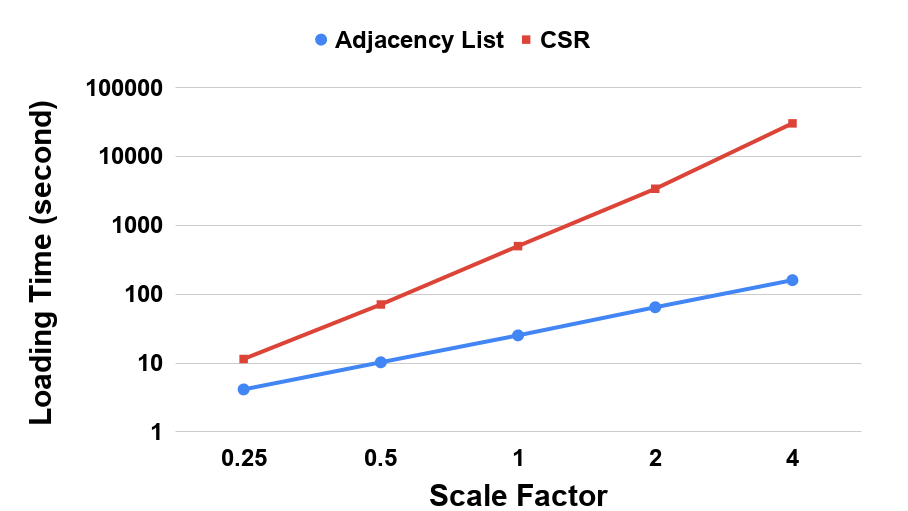
\includegraphics[width=0.8\textwidth]{pics/Scalability_Loading_GraphTopology.png}
        \label{fig:Scalability-Topology-Loading}
    }
\centering
    \subfigure[Change in memory footprint.]
    {
        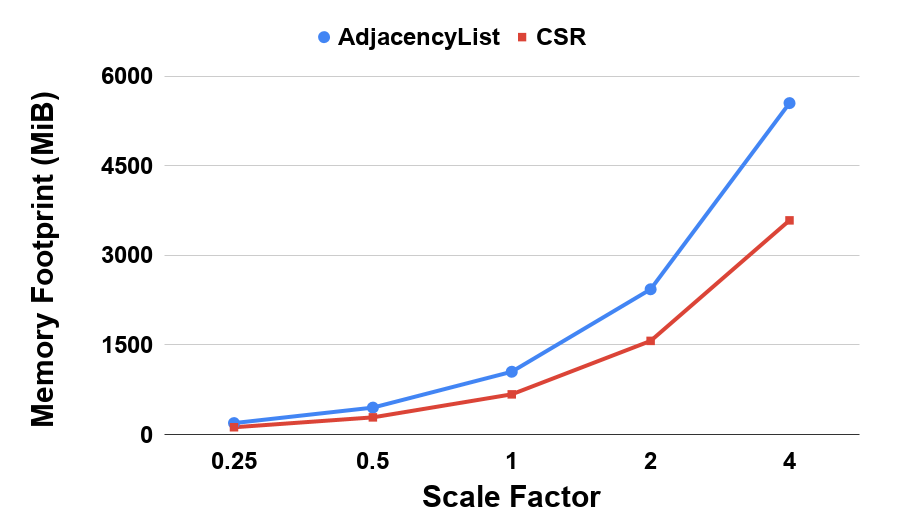
\includegraphics[width=0.8\textwidth]{pics/Scalability_Memory_GraphTopology.png}
        \label{fig:Scalability-Topology-Memory}
    }
    \caption{Effect of increasing data size on the scalability of graph topology structures.}
    \label{fig:Scalability-Topology}
\end{figure}


% Please add the following required packages to your document preamble:
% \usepackage{booktabs}
% \usepackage{multirow}
% \usepackage{graphicx}
\begin{table}[H]
\centering
\resizebox{\textwidth}{!}{%
\begin{tabular}{@{}|l||l|l|l||l|l|l|@{}}
\toprule
\multirow{2}{*}{Scale Factor} & \multicolumn{3}{c||}{Loading Time (Second)} & \multicolumn{3}{c|}{Memory Footprint (MiB)} \\ \cmidrule(l){2-7} 
 & Adjacency List & CSR & Adjacency Matrix & Adjacency List & CSR & Adjacency Matrix \\ \midrule
0.25 & 4 & 11 & 67 & 192 & 122 & 81,625 \\ \midrule
0.5 & 10 & 70 & N/A & 452 & 288 & N/A \\ \midrule
1 & 25 & 499 & N/A & 1,053 & 674 & N/A \\ \midrule
2 & 64 & 3,390 & N/A & 2,435 & 1,569 & N/A \\ \midrule
4 & 159 & 30,263 & N/A & 5,554 & 3,590 & N/A \\ \bottomrule
\end{tabular}%
}
\caption{Evaluation results of graph topology structures scalability.}
\label{tbl-EvalResults-Scal-Topology}
\end{table}

\section{Scalability}
\label{sec:eval-scalability}

In this section, we present the set of evaluation results for the experiments we conducted in order to evaluate the scalability of the different graph data structures. We evaluate the scalability of a graph data structure using two factors. Firstly, we evaluate the time taken to load the evaluation dataset into each of the graph data structures. Secondly, we measure the amount of memory consumed by each graph data structure in order to store the loaded data. We measure both the loading time and memory footprint when loading each scale factor of the evaluation dataset.  

In (\ref{subsec:scalability-topology}), we present the evaluation results concerning the scalability of the graph topology structures. We present the evaluation results concerning the scalability of the graph properties structures in (\ref{subsec:scalability-properties}).

\subsection{Scalability: Graph Topology Structures}
\label{subsec:scalability-topology}

In this section, we present the evaluation results regarding the scalability of the graph topology structures (adjacency list, compressed sparse row  (CSR), and adjacency matrix).

\begin{itemize}  

\item \textbf{Experiment Setup:}\\
In this experiment we used the batch data loader to load the evaluation dataset into the different graph topology structures. We fixed the batch size to 1000 record per batch. For each graph topology structure, we measured the loading time and memory footprint when loading each of the scale factors of the evaluation dataset. We executed each test for five to twenty times and recorded the loading time and memory footprint of each run. We took the average of the measured figures after removing the most top and least figures.

\item \textbf{Expected Result:}\\
We expect adjacency list to outperform adjacency matrix and compressed sparse row (CSR) and score the least loading time. We expect the loading time of adjacency matrix to be the largest among the three structures.

In regard to the memory footprint, we expect the memory footprint of adjacency matrix to be a lot bigger than the memory footprint of the adjacency list and the compressed sparse row (CSR). We expect the memory footprint of CSR to be smaller than that of adjacency list.

\item \textbf{Observation:}\\   
We observed that the loading time of adjacency list is increasing with an average rate of (2.5x) as we increase the scale factor of the loaded data. A higher average rate (7.3x) was recorded for the increase in loading time while we increase the scale factor of the loaded data into the compressed sparse row (CSR). We recorded a higher time taken in loading the CSR structure than that taken in loading the adjacency list across all the scale factors. The loading time of CSR was on average (54) times the loading time of adjacency list.

In regard to the memory footprint of stored data, we observed that the memory footprint of adjacency list is increasing with an average rate of (2.315x) as we increase the scale factor of the loaded data. A slightly higher average rate (2.329x) was recorded for the increase in memory footprint while we increase the scale factor of the loaded data into the compressed sparse row (CSR). In contrast to the difference in loading time between the adjacency list and the CSR structure, we recorded a higher memory footprint taken in storing the loaded data in the adjacency list than the memory footprint of storing the loaded data in the CSR structure across all the scale factors. The memory footprint of adjacency list was on average (1.56) times the memory footprint of CSR.

Concerning the adjacency matrix, we failed to load any of the scale factors of the evaluation dataset except for the smallest (0.25) scale factor. Loading the evaluation dataset with the (0.25) scale factor has consumed around 80 GiB. We ran out of memory trying to load the evaluation dataset with the (0.5) scale factor due to memory limitation of the machine used in running the evaluation experiments which is 128 GiB. However, the time taken to load the evaluation dataset with the (0.25) scale factor was (16) times the corresponding loading time of adjacency list and (6) times the loading time of CSR. Meanwhile, the memory footprint of the data stored in adjacency matrix was (425) times the corresponding memory footprint of adjacency list and (669) times the memory footprint of CSR.

In (\ref{fig:Scalability-Topology}), we show two graphs depicting the scalability of adjacency list and compressed sparse row in terms of loading time and memory footprint. In (Figure \ref{fig:Scalability-Topology-Loading}), we show a chart with the change in the loading time of each scale factor of the evaluation dataset into the adjacency list and the compressed sparse row (CSR). In (Figure \ref{fig:Scalability-Topology-Memory}), we show a chart with the change in the memory footprint of each scale factor of the evaluation dataset into the adjacency list and the compressed sparse row (CSR). In (\ref{tbl-EvalResults-Scal-Topology}), we present a table containing the exact figures we recorded for each of the scalability experiments we executed on the adjacency list, the compressed sparse row (CSR), and the adjacency matrix.

\item \textbf{Explanation:}\\
The (\texttt{std::vector}) data structure forces a data movement operation to occur for all the data following an inserted element in any place other than the end of the vector in order to free room for storing it. Both, compressed sparse row (CSR) and adjacency list are utilizing the (\texttt{std::vector}) data structure to store their data. However, as the loaded elements into the adjacency list are splitted up on several (\texttt{std::vector}) structures, the accumulative number of elements that needs to be displaced each time a new element comes is far fewer than in CSR, which in return causes the CSR structure to take more time in loading the data than the adjacency list. 

The \texttt{std::map}) data structure that is used by adjacency list and CSR has a complexity of ($O(log(n))$ for insertion which means as the number of elements stored in the data structure increases the insertion time will also increase. 

The increase in insertion time into the (\texttt{std::map}) participates into increasing the average rate of loading time to more than (2.0x) for both: adjacency list and CSR.

In regard to the memory footprint, the (\texttt{std::vector}) data structure which is utilized by compressed sparse row (CSR) and adjacency list to store their data is consuming extra memory in order to manage the container, besides the memory already consumed for storing the elements themselves. By using only two (\texttt{std::vector}) data structures in CSR the additional memory overhead is small and negligible to the memory consumed by the stored elements.On the contrary,the number of (\texttt{std::vector}) data structures used in adjacency list is equal to the number of vertices in the graph which makes explains the more memory consumed to store the data in comparison to the CSR structure.

The adjacency matrix memory consumption is much higher in comparison to CSR and adjacency list due to the memory requirements of adjacency matrix which is \mbox{($n^2$ bits)}, where "$n$" is the number of vertices in the graph. Also, the loading time of adjacency matrix is relatively high due to the need to expand each of the (\texttt{std::vector}) data structures of adjacency matrix every time a new element needs to be included into the matrix.

\item \textbf{Conclusion:}\\
To answer question number (1) from the evaluation questions listed in (\ref{sec:EvalQuests}), the evaluation results of the scalability of the three graph topology structures (adjacency list, compressed sparse roe (CSR), and adjacency matrix), are showing that the CSR structure is more suitable for use-cases where memory saving is the most important factor. However, adjacency list is offering a much better performance in terms of loading time with an average of (1.56) times the memory consumption of CSR. Lastly, adjacency matrix huge memory consumption makes it a poor scalable structure and makes it only useful for use-cases where the dataset is tiny.

\end{itemize}


\subsection{Scalability: Graph Properties Structures}
\label{subsec:scalability-properties}

In this section, we present the evaluation results regarding the scalability of the graph properties structures (universal table, emerging schema, and nested key-value store).

\begin{itemize}  

\item \textbf{Experiment Setup:}\\
In this experiment we used the batch data loader to load the evaluation dataset into the different graph properties structures. We fixed the batch size to 1000 record per batch. For each graph properties structure, we measured the loading time and memory footprint when loading each of the scale factors of the evaluation dataset. We executed each test for twenty times and recorded the loading time and memory footprint of each run. We took the average of the measured figures after removing the most top and least figures.


\begin{figure}[H]
\centering
    \subfigure[Change in loading time.]
    {
        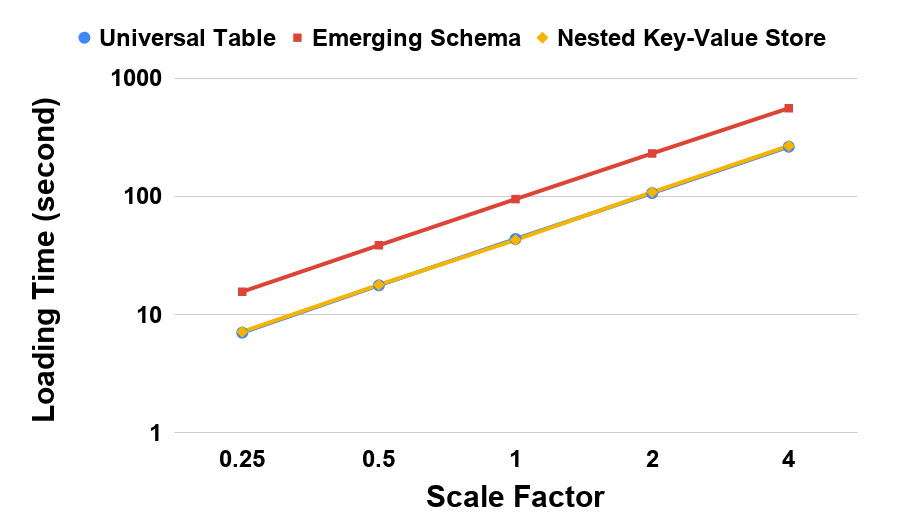
\includegraphics[width=0.85\textwidth]{pics/Scalability_Loading_GraphProperties.png}
        \label{fig:Scalability-Properties-Loading}
    }
\centering
    \subfigure[Change in memory footprint.]
    {
        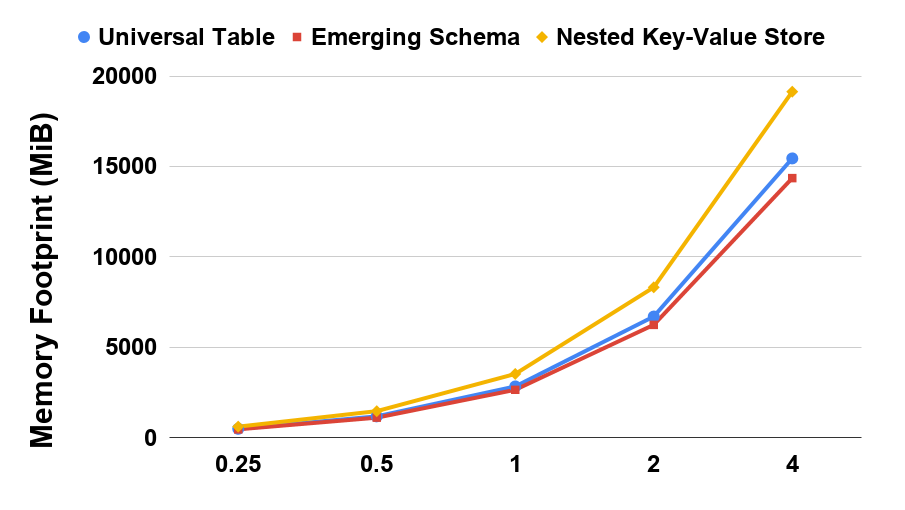
\includegraphics[width=0.85\textwidth]{pics/Scalability_Memory_GraphProperties.png}
        \label{fig:Scalability-Properties-Memory}
    }
    \caption{Effect of increasing data size on the scalability of graph properties structures.}
    \label{fig:Scalability-Properties}
\end{figure}


% Please add the following required packages to your document preamble:
% \usepackage{booktabs}
% \usepackage{multirow}
% \usepackage{graphicx}
\begin{table}[H]
\centering
\resizebox{\textwidth}{!}{%
\begin{tabular}{@{}|l||l|l|l||l|l|l|@{}}
\toprule
\multirow{2}{*}{Scale Factor} & \multicolumn{3}{c||}{Loading Time (Second)} & \multicolumn{3}{c|}{Memory Footprint (MiB)} \\ \cmidrule(l){2-7} 
 & Universal Table & Emerging Schema & Nested Key-Value Store & Universal Table & Emerging Schema & Nested Key-Value Store \\ \midrule
0.25 & 7 & 15 & 7 & 492 & 463 & 612 \\ \midrule
0.5 & 17 & 38 & 17 & 1,180 & 1,108 & 1,469 \\ \midrule
1 & 43 & 94 & 43 & 2,836 & 2,649 & 3,526 \\ \midrule
2 & 106 & 230 & 108 & 6,702 & 6,243 & 8,317 \\ \midrule
4 & 263 & 557 & 267 & 15,448 & 14,358 & 19,140 \\ \bottomrule
\end{tabular}%
}
\caption{Evaluation results of graph properties structures scalability.}
\label{tbl-EvalResults-Scal-Properties}
\end{table}


\item \textbf{Expected Result:}\\
We expect nested key-value store and universal table to record the same loading time of the datasets. We expect the loading time of emerging schema to be the larger than the loading time of nested key-value store and universal table.

In regard to the memory footprint, we expect the memory footprint of universal table to be the largest. We expect the memory footprint of emerging schema to be smaller than that of nested key-value store.


\item \textbf{Observation:}\\
We observed that the loading time of all the three graph properties structures (universal table, emerging schema, and nested key-value store) is increasing with the same average rate of (2.4x) as we increase the scale factor of the loaded data. We recorded that almost the same time was taken in loading the universal table and the nested key-value store with a slight advantage for the universal table when loading the evaluation dataset with scale factors (2 and 4). The loading time of emerging schema was on average (2.17) times the loading time of universal table.

In regard to the memory footprint of stored data, we observed that the memory footprint of all the three graph properties structures (universal table, emerging schema, and nested key-value store) is increasing with the same average rate of (2.4x) as we increase the scale factor of the loaded data which is the same average rate we recorded for the increase in the loading time. The emerging schema structure has recorded the lowest memory footprint among the three graph properties structures across all the evaluation dataset scale factors. In the second place came the universal table with a memory footprint that on average equals (1.07) times the memory footprint of emerging schema. The highest memory footprint was recorded for the nested key-value store with an average of (1.33) times the memory footprint of emerging schema and (1.24) times the memory footprint of universal table.

In (\ref{fig:Scalability-Properties}), we show two graphs depicting the scalability of universal table, emerging schema, and nested key-value store in terms of loading time and memory footprint. In (Figure \ref{fig:Scalability-Properties-Loading}), we show a chart with the change in the loading time of each scale factor of the evaluation dataset into the three graph properties structures and in (Figure \ref{fig:Scalability-Properties-Memory}), we show a chart with the change in the memory footprint. In (\ref{tbl-EvalResults-Scal-Properties}), we present a table containing the exact figures we recorded for each of the scalability experiments we executed on the universal table, emerging schema, and nested key-value store.

\item \textbf{Explanation:}\\
The (\texttt{std::map}) data structure that is used by universal table, emerging schema and nested key-value store has a complexity of ($O(log(n))$ for insertion which means as the number of elements stored in the data structure increases the insertion time will also increase. The increase in insertion time into the (\texttt{std::map}) participates into increasing the average rate of loading time to more than (2.0x) for the three graph properties structures.

The loading time in universal table and nested key-value store is almost equal because both data structure utilize the (\texttt{std::map}) data structure as their main container for storing the graph properties. The clustering operation that takes place after loading the data in emerging schema is causing the more loading time that emerging schema is taking in comparison to universal table and nested key-value store.

In regard to the memory footprint, nested key-value store has recorded the largest memory footprint among all the three graph topology structures due to the memory that is used to store the properties names in each and every row in addition to the properties values. The emerging schema structure has benefited form the vertical partitioning of the data into a set of column groups to record less memory footprint than that of universal table. The vertical partitioning used in emerging schema is reducing the memory consumption by eliminating most of the null values and not storing them.

\item \textbf{Conclusion:}\\
To answer question number (1) from the evaluation questions listed in (\ref{sec:EvalQuests}), the evaluation results of the scalability of the three graph properties structures (universal table, emerging schema, and nested key-value store), are showing that the emerging schema structure is more suitable for use-cases where memory saving is the most important factor, thanks to the vertical partitioning method it is using. However, universal table and nested key-value store are offering a better performance in terms of loading time.

\end{itemize}



\section{Batch Data Loading}
\label{sec:eval-batchLoading}

In this section, we present the evaluation results regarding the effect of batch size on the loading time of graph structures. Due to the scalability issue with adjacency matrix which we explained in (\ref{fig:Scalability-Topology}), we were not able to consider adjacency matrix in this test.

\begin{itemize}  

\item \textbf{Experiment Setup:}\\
In this experiment we used the batch data loader to load the evaluation dataset into the different graph structures. We loaded the data into each graph structure with batch sizes set to (1, 10, 100, 1000, 10000, and 100000). We used the evaluation dataset with scale factor (1) in this test. For each graph structure, we measured the loading time when loading the evaluation dataset using each of the of the batch sizes. We executed each test for ten to twenty times and recorded the loading time of each run. We took the average of the measured figures after removing the most top and least figures.


\item \textbf{Expected Result:}\\
For all graph structures we expect the loading time to decrease as we increase in batch size of the loaded data.



\begin{figure}[H]
\centering
    \subfigure[Change in loading time of graph topology structures.]
    {
        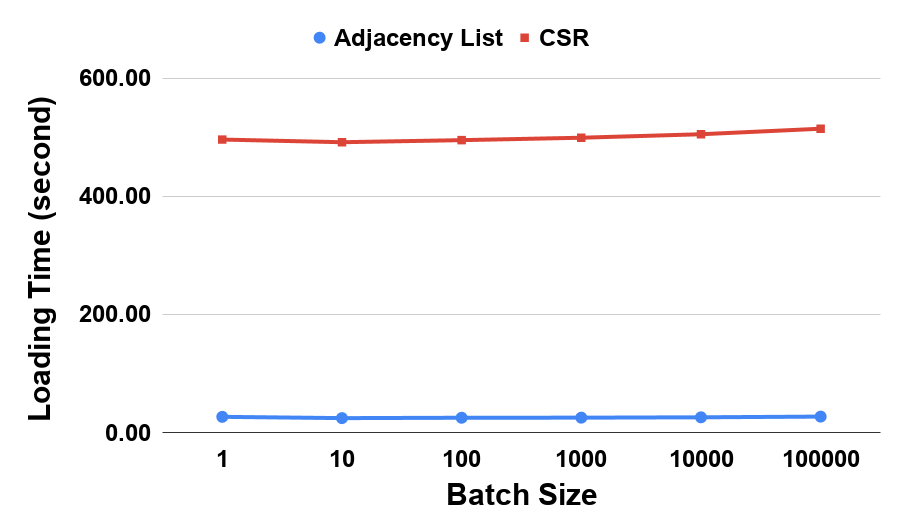
\includegraphics[width=0.75\textwidth]{pics/Batch_Loading_GraphTopology.png}
        \label{fig:Batch-Loading-Topology}
    }
\centering
    \subfigure[Change in loading time of graph properties structures.]
    {
        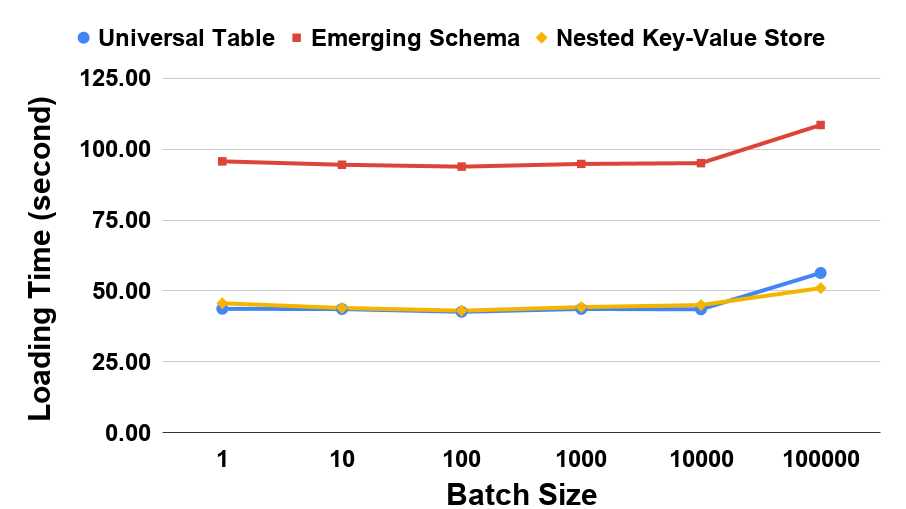
\includegraphics[width=0.75\textwidth]{pics/Batch_Loading_GraphProperties.png}
        \label{fig:Batch-Loading-Properties}
    }
    \caption{Effect of increasing batch size on the loading time of graph structures.}
    \label{fig:Batch-Loading}
\end{figure}


% Please add the following required packages to your document preamble:
% \usepackage{booktabs}
% \usepackage{multirow}
% \usepackage{graphicx}
\begin{table}[H]
\centering
\resizebox{\textwidth}{!}{%
\begin{tabular}{@{}|l||l|l||l|l|l|@{}}
\toprule
\multirow{2}{*}{Batch Size} & \multicolumn{2}{c||}{Graph Topology Structures} & \multicolumn{3}{c|}{Graph Properties Structures} \\ \cmidrule(l){2-6} 
 & Adjacency List & CSR & Universal Table & Emerging Schema & Nested Key-Value Store \\ \midrule
1 & 26.641 & 496.502 & 43.685 & 95.737 & 45.647 \\ \midrule
10 & 24.476 & 491.992 & 43.591 & 94.540 & 43.977 \\ \midrule
100 & 25.087 & 495.490 & 42.630 & 93.870 & 43.034 \\ \midrule
1000 & 25.247 & 499.597 & 43.636 & 94.831 & 44.282 \\ \midrule
10000 & 25.855 & 505.502 & 43.504 & 95.112 & 45.016 \\ \midrule
100000 & 27.046 & 514.883 & 56.338 & 108.571 & 50.994 \\ \bottomrule
\end{tabular}%
}
\caption{Evaluation results of batch loading time of graph structures in seconds.}
\label{tbl-EvalResults-Batch-Loading}
\end{table}


\item \textbf{Observation:}\\
We observed that by increasing the batch size, the change in loading time of all the graph structures was too small. The loading time for the graph topology structures started to decrease at first and recorded the lowest loading time when the batch size was set to (10) and then started to increase to record the highest loading time at (100000). Similar observation was made for graph properties structures as the loading time started to decrease at first and recorded the lowest loading time when the batch size was set to (100) and then started to increase to record the highest loading time at (100000).

In (\ref{fig:Batch-Loading}), we show two graphs depicting the change in loading time of the graph structure as an effect of the change in the batch size. In (Figure \ref{fig:Batch-Loading-Topology}), we show a chart with the change in the loading time that corresponds to each batch size of the data loaded into the graph topology structures and in (Figure \ref{fig:Batch-Loading-Properties}), we show a chart with the change in the loading time that corresponds to each batch size of the data loaded into the graph properties structures. In (\ref{tbl-EvalResults-Batch-Loading}), we present a table containing the exact figures we recorded for each of the batch loading experiments we executed on the graph structures.\\

\item \textbf{Explanation:}\\
Our expectation that the loading time will decrease as we increase the batch size was based on the number of times the batch loading procedure in (\ref{BatchDataLoader}) will need to push the buffer contents into the graph structure and then clear the buffer. The results was not fully consistent with our expectation.

We used the (\texttt{perf}) tool that is part of the (\texttt{ubuntu}) operating system to further analyze the performance of the tests from hardware perspective\footnote{For more information on the (\texttt{perf}) tool see: http://manpages.ubuntu.com/manpages/bionic/man1/perf.1.html}.\\


% Please add the following required packages to your document preamble:
% \usepackage{booktabs}
\begin{table}[H]
\centering
\begin{tabular}{@{}|l|l|l|@{}}
\toprule
Batch size & \# Buffer Flushes & Cache Misses (\%) \\ \midrule
1 & 15,530,170 & 10.848 \\ \midrule
10 & 1,553,017 & 10.923 \\ \midrule
100 & 155,302 & 11.639 \\ \midrule
1000 & 15,531 & 13.462 \\ \midrule
10000 & 1,553 & 18.542 \\ \midrule
100000 & 156 & 43.622 \\ \bottomrule
\end{tabular}
\caption{The change in the number of buffer flushes and the percentage of cache misses with the different batch sizes.}
\label{tbl:perf-analysis}
\end{table}

We observed in the statistics collected using the (\texttt{perf}) tool that the percentage of cache misses to the total number of cache references was increasing by the increase in the batch size. The copy of the buffer contents into the graph structure is the main source of the cache misses. The bigger the buffer size gets, the more it can't fit totally into the cache memory and the more cache misses we get.

The loading with smaller batch sizes has a better cache utilization with an average of only (10.84 \%) when we set the batch size to (1). However, the number of times we flush the buffer contents into the graph structure is the highest (15.5 million times on a batch size of (1)). On the contrary, the loading with larger batch sizes has a worse cache utilization with an average of (43.62 \%) when we set the batch size to (100000). However, the number of times we flush the buffer contents into the graph structure is the lowest (156 times on a batch size of (100000)).

The effect of the percentage of cache misses and the number of times we flush the buffer are contradicting each other. This leads to the decrease in loading time at the lower batch sizes when the cache misses are at its lowest and the increase in loading time at the larger batch sizes when the number of times we flush the buffer contents is the smallest.

We show in (\ref{tbl:perf-analysis}), the change in the number of times we flush the buffer as well as the percentage of cache misses caused by the change in batch size.


\item \textbf{Conclusion:}\\
To answer question number (2) from the evaluation questions listed in (\ref{sec:EvalQuests}), the evaluation results of the batch loading of the graph structures, are showing that there is a minimal effect for the batch size on the loading time. The minimal effect of batch size is because all the data is main memory resident and no disk storage is involved. The batch size setting need to be carefully tuned to reach the lowest loading time. In our experiments, we found the batch size (10) is providing the lowest loading time for the graph topology structures and the batch size (100) is providing the lowest loading time for the graph properties structures. 

\end{itemize}

\section{Parallel Data Loading}
\label{sec:eval-parallelLoading}

In this section, we present the evaluation results regarding the effect of parallel loading on the loading time of parallel adjacency list and parallel nested key-value store.

\begin{itemize}

\item \textbf{Experiment Setup:}\\
In this experiment we used the parallel data loader to load the evaluation dataset into the parallel adjacency list and the parallel nested key-value store structures. We executed the loading with a parallelism degree of (1, 2, 4, 8, and 16). We fixed the buffer size of the parallel loader to (1000). We loaded the evaluation dataset with scale factor (1). We executed each test for twenty times and recorded the loading time of each run. We took the average of the measured figures after removing the most top and least figures.



\begin{figure}[H]
\centering
    \subfigure[Change in loading time of parallel adjacency list.]
    {
        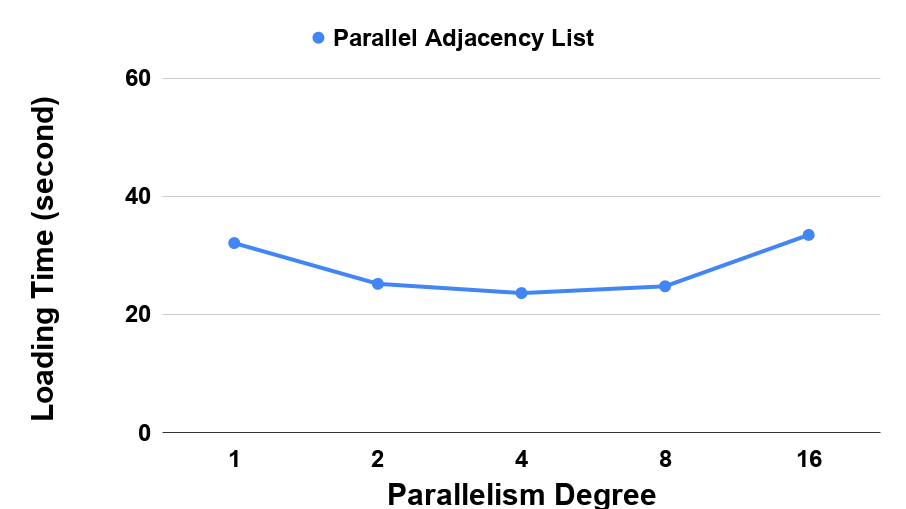
\includegraphics[width=0.7\textwidth]{pics/Parallel_Loading_AdjLst.png}
        \label{fig:Parallel-Loading-AdjLst}
    }
\centering
    \subfigure[Change in loading time of parallel nested key-value store.]
    {
        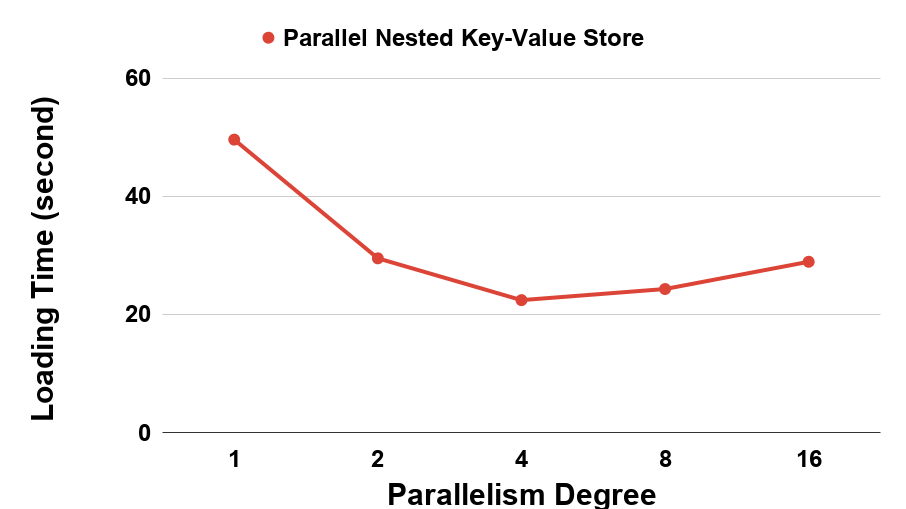
\includegraphics[width=0.7\textwidth]{pics/Parallel_Loading_NestedStore.png}
        \label{fig:Parallel-Loading-NestedStore}
    }
    \caption{Degree of parallelism effect on the loading time of parallel adjacency list and parallel nested key-value store.}
    \label{fig:Parallel-Loading}
\end{figure}



\begin{table}[H]
\centering
%\resizebox{\textwidth}{!}{%
\begin{tabular}{@{}|l||l|l|@{}}
\toprule
\multicolumn{1}{|c||}{Parallelism Degree} & Parallel Adjacency List & Parallel Nested Key-Value Store \\ \midrule
1 & 32.109 & 49.638\\ \midrule
2 & 25.205 & 29.524 \\ \midrule
4 & 23.632 & 22.439 \\ \midrule
8 & 24.784 & 24.324 \\ \midrule
16 & 33.492 & 28.941 \\ \bottomrule
\end{tabular}%
%}
\caption{Evaluation results for time of parallel loading of the parallel adjacency list and the parallel nested key-value store in seconds.}
\label{tbl-EvalResults-Parallel-Loading}
\end{table}





% Please add the following required packages to your document preamble:
% \usepackage{booktabs}
% \usepackage{multirow}
% \usepackage{graphicx}
%\begin{table}[H]
%\centering
%\resizebox{\textwidth}{!}{%
%\begin{tabular}{@{}|l||l|l|l||l|l|l|@{}}
%\toprule
%\multirow{2}{*}{Parallelism Degree} & \multicolumn{3}{c||}{Adjacency %List} & \multicolumn{3}{c|}{Nested Key-Value Store} \\ %\cmidrule(l){2-7} 
 %& Scale Factor (0.25) & Scale Factor (1) & Scale Factor (4) & Scale Factor (0.25) & Scale Factor (1) & Scale Factor (4) \\ \midrule
%1 & 5.041 & 32.109 & 199.987 & 8.030 & 49.638 & 311.251 \\ \midrule
%2 & 4.143 & 25.205 & 148.196 & 4.811 & 29.524 & 180.038 \\ \midrule
%4 & 3.862 & 23.632 & 134.912 & 3.446 & 22.439 & 143.121 \\ \midrule
%8 & 4.200 & 24.784 & 139.006 & 3.687 & 24.324 & 159.772 \\ \midrule
%16 & 5.408 & 33.492 & 195.444 & 4.433 & 28.941 & 186.111 \\ %\bottomrule
%\end{tabular}%
%}
%\caption{Evaluation results for time of parallel loading of the %parallel adjacency list and the parallel nested key-value store in %seconds.}
%\label{tbl-EvalResults-Parallel-Loading}
%\end{table}



\item \textbf{Expected Result:}\\
We expect the loading time of parallel adjacency list and parallel nested key-value store to decrease as we increase in batch size of the loaded data.


\item \textbf{Observation:}\\
We observed that by increasing the parallelism degree, the loading time of parallel adjacency list and parallel nested key-value store decreases just until we reach the parallelism degree of (4). On parallelism degree (4), the two parallel graph structures scored their least loading time. However, the loading time of both graph structures has started to increase once we set the parallelism degree higher than (4).

With the parallelism degree set to (4), the loading time of parallel adjacency list was less by (6 to 16\%) than the corresponding loading time of the sequential version of adjacency list. The parallel nested key-value store has scored a loading time that is less by (47 to 52\%) than the corresponding loading time of the sequential version of nested key-value store, also with the parallelism degree set to (4).

On parallelism degree (1), both: the parallel adjacency list and the parallel nested key-value store recorded a loading time that is higher than the corresponding loading time of the sequential version.

In (\ref{fig:Parallel-Loading}), we show two graphs depicting the change in loading time of parallel adjacency list and parallel nested key-value store as an effect of the change in the parallelism degree of the parallel loader. In (Figure \ref{fig:Parallel-Loading-AdjLst}), we show a chart with the change in the loading time that corresponds to each degree of parallelism when loading the evaluation dataset with scale factor (1) into the parallel adjacency list and in (Figure \ref{fig:Parallel-Loading-NestedStore}), we show a similar chart for the change in the loading time of the parallel nested key-value store. In (\ref{tbl-EvalResults-Parallel-Loading}), we present a table containing the exact figures we recorded for each of the parallel loading experiments we executed on the parallel adjacency and the parallel nested key-value store.

\item \textbf{Explanation:}\\
The observed behaviour of decrease in the loading time as we increase the parallelism degree only up to the parallel degree of (4) is due to the maximum ability of the physical machine processor to execute only (4) threads in parallel. Increasing the number of threads to more than (4) has caused the loading time to increase due to the overhead of synchronization required to be done by the operating system between the threads in order to execute the instructions of all threads.

\item \textbf{Conclusion:}\\
To answer question number (3) from the evaluation questions listed in (\ref{sec:EvalQuests}), the evaluation results are showing that the parallel loading of data into the parallel adjacency list and the parallel nested key-value store has decreased the loading time by (6 to 16\%) for the parallel adjacency list and (47 to 52\%) for the parallel nested key-value store over their sequential counterparts. 

The maximum decrease in loading time was achieved when the parallelism degree was set to (4). The correct choice of parallelism degree should be configured according to the parallelism capabilities of the processor.

\end{itemize}


\section{Summary}
\label{sec:eval-summary_part1}

In this chapter, we presented the first part of our evaluation results, with which we answered the evaluation questions number 1, 2, and 3 stated in (\ref{sec:EvalQuests}). We presented the loading time and memory footprint scalability test for the different graph structures. We presented the effect of batch size on the loading time of graph structures. We showed the possible improvement that parallel loading of data can introduce over sequential loading.

In next chapter, we present the second and last part of our evaluation results, with which we will answer the evaluation question number 4 stated in (\ref{sec:EvalQuests}).


}